% ============================================================
%  ANNOTATION — Euclidean Geometry in Mathematical Olympiads
%  Evan Chen (2016)
%  Compile: latexmk -pdf evan-chen-egmo.tex
%  Figures: uses tikz + tkz-euclide
% ============================================================

\documentclass[11pt, letterpaper]{article}

\usepackage[margin=1.2in]{geometry}
\usepackage{amsmath, amssymb, amsthm}
\usepackage{mathtools}
\usepackage{hyperref}
\usepackage{enumitem}
\usepackage{parskip}
\usepackage{microtype}
\usepackage{xcolor}

% ── Geometry figure packages ────────────────────────────────
\usepackage{tikz}
\usepackage{tkz-euclide}          % high-level Euclidean geometry
\usetikzlibrary{calc, angles, quotes, intersections, through}

% ── Theorem environments ─────────────────────────────────────
\newtheorem{theorem}{Theorem}[section]
\newtheorem{lemma}[theorem]{Lemma}
\newtheorem{proposition}[theorem]{Proposition}
\newtheorem{corollary}[theorem]{Corollary}
\theoremstyle{definition}
\newtheorem{definition}[theorem]{Definition}
\newtheorem{example}[theorem]{Example}
\newtheorem{problem}{Problem}[section]
\theoremstyle{remark}
\newtheorem*{remark}{Remark}
\newtheorem*{note}{Note}

% ── Geometry macros ──────────────────────────────────────────
\newcommand{\seg}[1]{\overline{#1}}
\newcommand{\ray}[1]{\overrightarrow{#1}}
\newcommand{\arc}[1]{\widehat{#1}}
\newcommand{\dang}{\measuredangle}          % directed angle
\newcommand{\cyclic}[1]{#1 \text{ cyclic}}
\newcommand{\pow}[2]{\mathrm{pow}(#1,\,#2)}
\newcommand{\rad}{\mathrm{rad}}

% Standard math shortcuts
\newcommand{\R}{\mathbb{R}}
\newcommand{\abs}[1]{\left|#1\right|}

% ── Document metadata ────────────────────────────────────────
\title{Euclidean Geometry in Mathematical Olympiads \\ \large Annotations \& Notes}
\author{Andre Ruiz Loera \\ \small \textit{Math}}
\date{Read: 2026}

% ============================================================
\begin{document}
\maketitle
\tableofcontents
\newpage

% ── OVERVIEW ────────────────────────────────────────────────
\section{Overview}

\textit{Euclidean Geometry in Mathematical Olympiads} (EGMO) by Evan Chen is the
standard olympiad geometry reference. It covers the full toolkit: angle chasing,
power of a point, radical axes, inversion, projective geometry, and more --- each
chapter ending with a curated problem set. The writing is unusually clean for a
competition math text.

% ── CHAPTER NOTES ───────────────────────────────────────────
\section{Chapter Notes}

% ────────────────────────────────────────────────────────────
\subsection{Chapter 1 — Angle Chasing}

\begin{definition}
  The \textbf{directed angle} $\dang(AB, CD)$ is the angle of rotation from
  line $AB$ to line $CD$, taken modulo $180^\circ$.
\end{definition}

\begin{theorem}[Inscribed Angle Theorem]
  Let $\omega$ be a circle with center $O$, and let $A$, $B$, $P$ lie on
  $\omega$ with $P$ not on arc $AB$. Then $\dang APB = \dang AOB / 2$.
  Equivalently, all inscribed angles subtending the same arc are equal.
\end{theorem}

% Example figure — triangle with circumcircle
\begin{center}
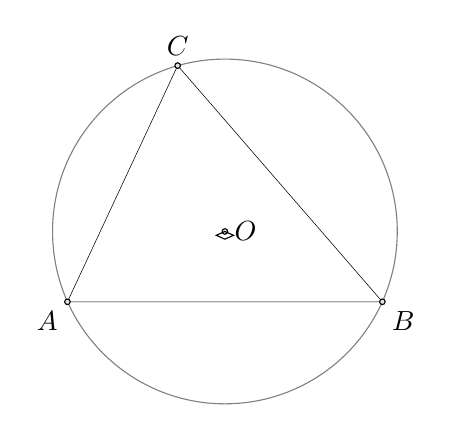
\begin{tikzpicture}[scale=2]
  % Define triangle vertices
  \tkzDefPoint(0,0){A}
  \tkzDefPoint(2,0){B}
  \tkzDefPoint(0.7,1.5){C}

  % Circumcircle
  \tkzCircumCenter(A,B,C)\tkzGetPoint{O}
  \tkzDrawCircle[thin, gray](O,A)

  % Triangle
  \tkzDrawPolygon(A,B,C)
  \tkzDrawPoints(A,B,C,O)
  \tkzLabelPoints[below left](A)
  \tkzLabelPoints[below right](B)
  \tkzLabelPoints[above](C)
  \tkzLabelPoints[right](O)

  % Mark circumcenter
  \tkzMarkRightAngle[size=0.06](A,O,B)
\end{tikzpicture}
\end{center}

\begin{remark}
  Use directed angles to avoid case splits. $\dang APB = \dang AQB$ iff
  $A$, $P$, $Q$, $B$ are concyclic.
\end{remark}

% ────────────────────────────────────────────────────────────
\subsection{Chapter 2 — Circles}

\begin{definition}
  The \textbf{power of a point} $P$ with respect to circle $\omega$ with
  center $O$ and radius $r$ is
  \[
    \pow{P}{\omega} = PO^2 - r^2.
  \]
  If a line through $P$ meets $\omega$ at $X$ and $Y$, then
  $\pow{P}{\omega} = \overline{PX} \cdot \overline{PY}$ (signed).
\end{definition}

\begin{theorem}[Radical Axis]
  The locus of points with equal power with respect to two circles is a line
  perpendicular to the line through their centers. The radical axes of three
  circles taken pairwise are concurrent (the \textbf{radical center}).
\end{theorem}

% Example figure — two circles with radical axis
\begin{center}
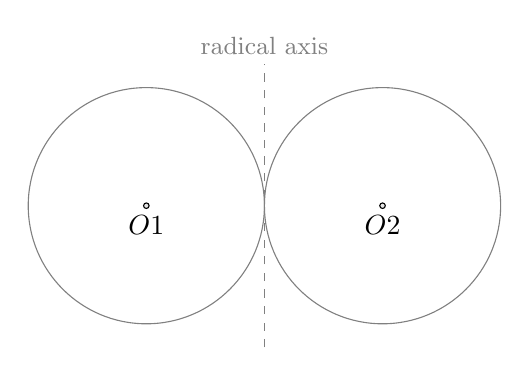
\begin{tikzpicture}[scale=1.2]
  \tkzDefPoint(0,0){O1}
  \tkzDefPoint(2.5,0){O2}
  \tkzDefPoint(1.25,0){M}   % midpoint, radical axis passes through here

  \tkzDrawCircle[thin](O1,M)
  \tkzDrawCircle[thin](O2,M)

  % Radical axis (vertical line at x=1.25 for equal radii)
  \draw[dashed, gray] (1.25,-1.5) -- (1.25,1.5) node[above, font=\small]{radical axis};

  \tkzDrawPoints(O1,O2)
  \tkzLabelPoints[below](O1,O2)
\end{tikzpicture}
\end{center}

% ────────────────────────────────────────────────────────────
\subsection{Chapter 3 — Lengths and Ratios}

Key tools: Stewart's Theorem, mass point geometry, Menelaus, Ceva.

\begin{theorem}[Ceva's Theorem]
  Cevians $AD$, $BE$, $CF$ of triangle $ABC$ are concurrent iff
  \[
    \frac{AF}{FB} \cdot \frac{BD}{DC} \cdot \frac{CE}{EA} = 1.
  \]
\end{theorem}

\begin{theorem}[Menelaus' Theorem]
  Points $D$, $E$, $F$ on lines $BC$, $CA$, $AB$ are collinear iff
  \[
    \frac{AF}{FB} \cdot \frac{BD}{DC} \cdot \frac{CE}{EA} = -1
    \quad \text{(signed ratios)}.
  \]
\end{theorem}

% ────────────────────────────────────────────────────────────
\subsection{Chapter 4 — Assorted Configurations}

Notable configurations to internalize:
\begin{itemize}
  \item Simson line
  \item Nine-point circle
  \item Orthocenter reflection over midpoint lies on circumcircle
  \item Miquel's theorem
  \item Spiral similarities
\end{itemize}

% ────────────────────────────────────────────────────────────
\subsection{Chapter 5 — Classical Geometry Revisited}

\begin{theorem}[Ptolemy's Theorem]
  For a cyclic quadrilateral $ABCD$,
  \[
    AC \cdot BD = AB \cdot CD + AD \cdot BC.
  \]
\end{theorem}

% ────────────────────────────────────────────────────────────
\subsection{Chapter 6 — Inversive Geometry}

\begin{definition}
  \textbf{Inversion} with center $O$ and radius $r$ maps a point $P \neq O$
  to the point $P'$ on ray $OP$ with $OP \cdot OP' = r^2$.
\end{definition}

Key facts:
\begin{itemize}
  \item Lines/circles through $O$ map to lines not through $O$, and vice versa.
  \item Circles not through $O$ map to circles not through $O$.
  \item Inversion preserves angles (it is conformal).
  \item Use inversion to kill tangency conditions.
\end{itemize}

% ── EXERCISES / PROBLEMS ────────────────────────────────────
\section{Exercises \& Problems}

\begin{problem}
  Let $ABC$ be a triangle with circumcircle $\omega$. The angle bisector from
  $A$ meets $\omega$ again at $M$. Show $MB = MC$.
\end{problem}

\begin{proof}
  Since $AM$ bisects $\angle BAC$, we have $\dang BAM = \dang CAM$.
  By the inscribed angle theorem, $\dang BAM = \dang BCM$ and
  $\dang CAM = \dang CBM$, so $\dang BCM = \dang CBM$, giving $MB = MC$.
\end{proof}

% ── TAKEAWAYS ───────────────────────────────────────────────
\section{Takeaways}

\begin{itemize}
  \item Use directed angles by default to eliminate case splits in circle problems.
  \item Power of a point + radical axis is the engine of most circle configuration problems.
  \item Inversion with center at a point of tangency almost always simplifies.
  \item Ceva and Menelaus are the right tools whenever concurrence/collinearity
        involves ratios on the sides of a triangle.
\end{itemize}

\end{document}
